\documentclass[]{book}
\usepackage{lmodern}
\usepackage{amssymb,amsmath}
\usepackage{ifxetex,ifluatex}
\usepackage{fixltx2e} % provides \textsubscript
\ifnum 0\ifxetex 1\fi\ifluatex 1\fi=0 % if pdftex
  \usepackage[T1]{fontenc}
  \usepackage[utf8]{inputenc}
\else % if luatex or xelatex
  \ifxetex
    \usepackage{mathspec}
  \else
    \usepackage{fontspec}
  \fi
  \defaultfontfeatures{Ligatures=TeX,Scale=MatchLowercase}
\fi
% use upquote if available, for straight quotes in verbatim environments
\IfFileExists{upquote.sty}{\usepackage{upquote}}{}
% use microtype if available
\IfFileExists{microtype.sty}{%
\usepackage{microtype}
\UseMicrotypeSet[protrusion]{basicmath} % disable protrusion for tt fonts
}{}
\usepackage[margin=1in]{geometry}
\usepackage{hyperref}
\hypersetup{unicode=true,
            pdftitle={Introducción al software R},
            pdfauthor={Paccioretti Pablo; Bruno Cecilia; Nores María Laura; Gonzalez Aldana},
            pdfborder={0 0 0},
            breaklinks=true}
\urlstyle{same}  % don't use monospace font for urls
\usepackage{natbib}
\bibliographystyle{apalike}
\usepackage{color}
\usepackage{fancyvrb}
\newcommand{\VerbBar}{|}
\newcommand{\VERB}{\Verb[commandchars=\\\{\}]}
\DefineVerbatimEnvironment{Highlighting}{Verbatim}{commandchars=\\\{\}}
% Add ',fontsize=\small' for more characters per line
\usepackage{framed}
\definecolor{shadecolor}{RGB}{248,248,248}
\newenvironment{Shaded}{\begin{snugshade}}{\end{snugshade}}
\newcommand{\KeywordTok}[1]{\textcolor[rgb]{0.13,0.29,0.53}{\textbf{#1}}}
\newcommand{\DataTypeTok}[1]{\textcolor[rgb]{0.13,0.29,0.53}{#1}}
\newcommand{\DecValTok}[1]{\textcolor[rgb]{0.00,0.00,0.81}{#1}}
\newcommand{\BaseNTok}[1]{\textcolor[rgb]{0.00,0.00,0.81}{#1}}
\newcommand{\FloatTok}[1]{\textcolor[rgb]{0.00,0.00,0.81}{#1}}
\newcommand{\ConstantTok}[1]{\textcolor[rgb]{0.00,0.00,0.00}{#1}}
\newcommand{\CharTok}[1]{\textcolor[rgb]{0.31,0.60,0.02}{#1}}
\newcommand{\SpecialCharTok}[1]{\textcolor[rgb]{0.00,0.00,0.00}{#1}}
\newcommand{\StringTok}[1]{\textcolor[rgb]{0.31,0.60,0.02}{#1}}
\newcommand{\VerbatimStringTok}[1]{\textcolor[rgb]{0.31,0.60,0.02}{#1}}
\newcommand{\SpecialStringTok}[1]{\textcolor[rgb]{0.31,0.60,0.02}{#1}}
\newcommand{\ImportTok}[1]{#1}
\newcommand{\CommentTok}[1]{\textcolor[rgb]{0.56,0.35,0.01}{\textit{#1}}}
\newcommand{\DocumentationTok}[1]{\textcolor[rgb]{0.56,0.35,0.01}{\textbf{\textit{#1}}}}
\newcommand{\AnnotationTok}[1]{\textcolor[rgb]{0.56,0.35,0.01}{\textbf{\textit{#1}}}}
\newcommand{\CommentVarTok}[1]{\textcolor[rgb]{0.56,0.35,0.01}{\textbf{\textit{#1}}}}
\newcommand{\OtherTok}[1]{\textcolor[rgb]{0.56,0.35,0.01}{#1}}
\newcommand{\FunctionTok}[1]{\textcolor[rgb]{0.00,0.00,0.00}{#1}}
\newcommand{\VariableTok}[1]{\textcolor[rgb]{0.00,0.00,0.00}{#1}}
\newcommand{\ControlFlowTok}[1]{\textcolor[rgb]{0.13,0.29,0.53}{\textbf{#1}}}
\newcommand{\OperatorTok}[1]{\textcolor[rgb]{0.81,0.36,0.00}{\textbf{#1}}}
\newcommand{\BuiltInTok}[1]{#1}
\newcommand{\ExtensionTok}[1]{#1}
\newcommand{\PreprocessorTok}[1]{\textcolor[rgb]{0.56,0.35,0.01}{\textit{#1}}}
\newcommand{\AttributeTok}[1]{\textcolor[rgb]{0.77,0.63,0.00}{#1}}
\newcommand{\RegionMarkerTok}[1]{#1}
\newcommand{\InformationTok}[1]{\textcolor[rgb]{0.56,0.35,0.01}{\textbf{\textit{#1}}}}
\newcommand{\WarningTok}[1]{\textcolor[rgb]{0.56,0.35,0.01}{\textbf{\textit{#1}}}}
\newcommand{\AlertTok}[1]{\textcolor[rgb]{0.94,0.16,0.16}{#1}}
\newcommand{\ErrorTok}[1]{\textcolor[rgb]{0.64,0.00,0.00}{\textbf{#1}}}
\newcommand{\NormalTok}[1]{#1}
\usepackage{longtable,booktabs}
\usepackage{graphicx,grffile}
\makeatletter
\def\maxwidth{\ifdim\Gin@nat@width>\linewidth\linewidth\else\Gin@nat@width\fi}
\def\maxheight{\ifdim\Gin@nat@height>\textheight\textheight\else\Gin@nat@height\fi}
\makeatother
% Scale images if necessary, so that they will not overflow the page
% margins by default, and it is still possible to overwrite the defaults
% using explicit options in \includegraphics[width, height, ...]{}
\setkeys{Gin}{width=\maxwidth,height=\maxheight,keepaspectratio}
\IfFileExists{parskip.sty}{%
\usepackage{parskip}
}{% else
\setlength{\parindent}{0pt}
\setlength{\parskip}{6pt plus 2pt minus 1pt}
}
\setlength{\emergencystretch}{3em}  % prevent overfull lines
\providecommand{\tightlist}{%
  \setlength{\itemsep}{0pt}\setlength{\parskip}{0pt}}
\setcounter{secnumdepth}{5}
% Redefines (sub)paragraphs to behave more like sections
\ifx\paragraph\undefined\else
\let\oldparagraph\paragraph
\renewcommand{\paragraph}[1]{\oldparagraph{#1}\mbox{}}
\fi
\ifx\subparagraph\undefined\else
\let\oldsubparagraph\subparagraph
\renewcommand{\subparagraph}[1]{\oldsubparagraph{#1}\mbox{}}
\fi

%%% Use protect on footnotes to avoid problems with footnotes in titles
\let\rmarkdownfootnote\footnote%
\def\footnote{\protect\rmarkdownfootnote}

%%% Change title format to be more compact
\usepackage{titling}

% Create subtitle command for use in maketitle
\newcommand{\subtitle}[1]{
  \posttitle{
    \begin{center}\large#1\end{center}
    }
}

\setlength{\droptitle}{-2em}

  \title{Introducción al software R}
    \pretitle{\vspace{\droptitle}\centering\huge}
  \posttitle{\par}
  \subtitle{Notas de clases}
  \author{Paccioretti Pablo\footnote{\href{mailto:pablopaccioretti@agro.unc.edu.ar}{\nolinkurl{pablopaccioretti@agro.unc.edu.ar}}} \\ Bruno Cecilia\footnote{\href{mailto:cebruno@agro.unc.edu.ar}{\nolinkurl{cebruno@agro.unc.edu.ar}}} \\ Nores María Laura\footnote{\href{mailto:lalinores@yahoo.com.ar}{\nolinkurl{lalinores@yahoo.com.ar}}} \\ Gonzalez Aldana\footnote{\href{mailto:aldanagonzalez@gmail.com}{\nolinkurl{aldanagonzalez@gmail.com}}}}
    \preauthor{\centering\large\emph}
  \postauthor{\par}
    \date{}
    \predate{}\postdate{}
  
\usepackage[utf8]{inputenc}
\usepackage{graphicx}
\usepackage{booktabs}
\usepackage{longtable}
\usepackage{framed,color}
\definecolor{shadecolor}{RGB}{248,248,248}
\usepackage{polyglossia}
\setmainlanguage{spanish}
\AtBeginDocument{\renewcommand{\chaptername}{Sección}}
\usepackage{longtable}


\usepackage{letltxmacro}
\LetLtxMacro\SavedIncludeGraphics\includegraphics
\def\includegraphics#1#{% #1 catches optional stuff (star/opt. arg.)
	\IncludeGraphicsAux{#1}%
}%
\newcommand*{\IncludeGraphicsAux}[2]{%
	\XeTeXLinkBox{%
		\SavedIncludeGraphics#1{#2}%
	}%
}%

\newenvironment{rmdblock}[1]
{\begin{shaded*}
		\begin{itemize}
			\renewcommand{\labelitemi}{
				\raisebox{-.7\height}[0pt][0pt]{
					{\setkeys{Gin}{width=3em,keepaspectratio}\includegraphics{images/#1}}
				}
			}
			\item
		}
		{
		\end{itemize}
	\end{shaded*}
}
\newenvironment{rmdnote}
{\begin{rmdblock}{note}}
	{\end{rmdblock}}
\newenvironment{rmdcaution}
{\begin{rmdblock}{caution}}
	{\end{rmdblock}}
\newenvironment{rmdimportant}
{\begin{rmdblock}{important}}
	{\end{rmdblock}}
\newenvironment{rmdtip}
{\begin{rmdblock}{tip}}
	{\end{rmdblock}}
\newenvironment{rmdwarning}
{\begin{rmdblock}{warning}}
	{\end{rmdblock}}

\usepackage{environ}
\usepackage{xcolor}
\NewEnviron{boxeda}%
  {\begin{center}%
   \noindent\fcolorbox{black}{gray!30}%
     {\parbox{33em}%
       {\vspace{15pt}\par
        \BODY
        \vspace{15pt}\par
       }%
     }%
   \end{center}%
  }
  
% \newenvironment{boxeda}
%     {\begin{center}
%       \begin{tabular}{|p{0.9\textwidth}|}
%        %\hline\\
%     }
%     { 
%     %\\\\\hline
%     \end{tabular} 
%     \end{center}
%     }

% \usepackage{booktabs}
% \usepackage{longtable}
% \usepackage{framed,color}
% \definecolor{shadecolor}{RGB}{248,248,248}
% 
% \ifxetex
%   \usepackage{letltxmacro}
%   \setlength{\XeTeXLinkMargin}{1pt}
%   \LetLtxMacro\SavedIncludeGraphics\includegraphics
%   \def\includegraphics#1#{% #1 catches optional stuff (star/opt. arg.)
%     \IncludeGraphicsAux{#1}%
%   }%
%   \newcommand*{\IncludeGraphicsAux}[2]{%
%     \XeTeXLinkBox{%
%       \SavedIncludeGraphics#1{#2}%
%     }%
%   }%
% \fi
% 
% \newenvironment{rmdblock}[1]
%   {\begin{shaded*}
%   \begin{itemize}
%   \renewcommand{\labelitemi}{
%     \raisebox{-.7\height}[0pt][0pt]{
%       {\setkeys{Gin}{width=3em,keepaspectratio}\includegraphics{images/#1}}
%     }
%   }
%   \item
%   }
%   {
%   \end{itemize}
%   \end{shaded*}
%   }
% \newenvironment{rmdnote}
%   {\begin{rmdblock}{note}}
%   {\end{rmdblock}}
% \newenvironment{rmdcaution}
%   {\begin{rmdblock}{caution}}
%   {\end{rmdblock}}
% \newenvironment{rmdimportant}
%   {\begin{rmdblock}{important}}
%   {\end{rmdblock}}
% \newenvironment{rmdtip}
%   {\begin{rmdblock}{tip}}
%   {\end{rmdblock}}
% \newenvironment{rmdwarning}
%   {\begin{rmdblock}{warning}}
%   {\end{rmdblock}}

\begin{document}
\maketitle

{
\setcounter{tocdepth}{1}
\tableofcontents
}
\hypertarget{instalacion-de-programas}{%
\chapter{Instalación de programas}\label{instalacion-de-programas}}

R puede ser instalado en múltiples plataformas tales como Windows, Mac
OS y en sistemas basados en Linux. Además hay múltiples entornos de
desarrollo integrado (\emph{Integrated Development Environment} IDE) los
cuales facilitan la programación. Ejemplos de este tipo de software es
el intérprete de R que contiene InfoStat \citep{Infostat} y RStudio
\citep{Rstudio}. Las interfaces gráficas de ambos softwares son
similares.

Links para las descargas:

\begin{itemize}
\tightlist
\item
  \href{https://cran.r-project.org/bin/windows/base/}{R (windows)}
\item
  \href{http://www.infostat.com.ar/descargas/demo/infostatinstaller_esp.exe}{InfoStat}
\end{itemize}

\hypertarget{breve-introduccion-a-la-interfaz-del-interprete-de-infostat}{%
\section{Breve introducción a la interfaz del intérprete de
InfoStat}\label{breve-introduccion-a-la-interfaz-del-interprete-de-infostat}}

La interfaz del intérprete de R en InfoStat se divide en cuatro paneles.

\begin{figure}
\centering
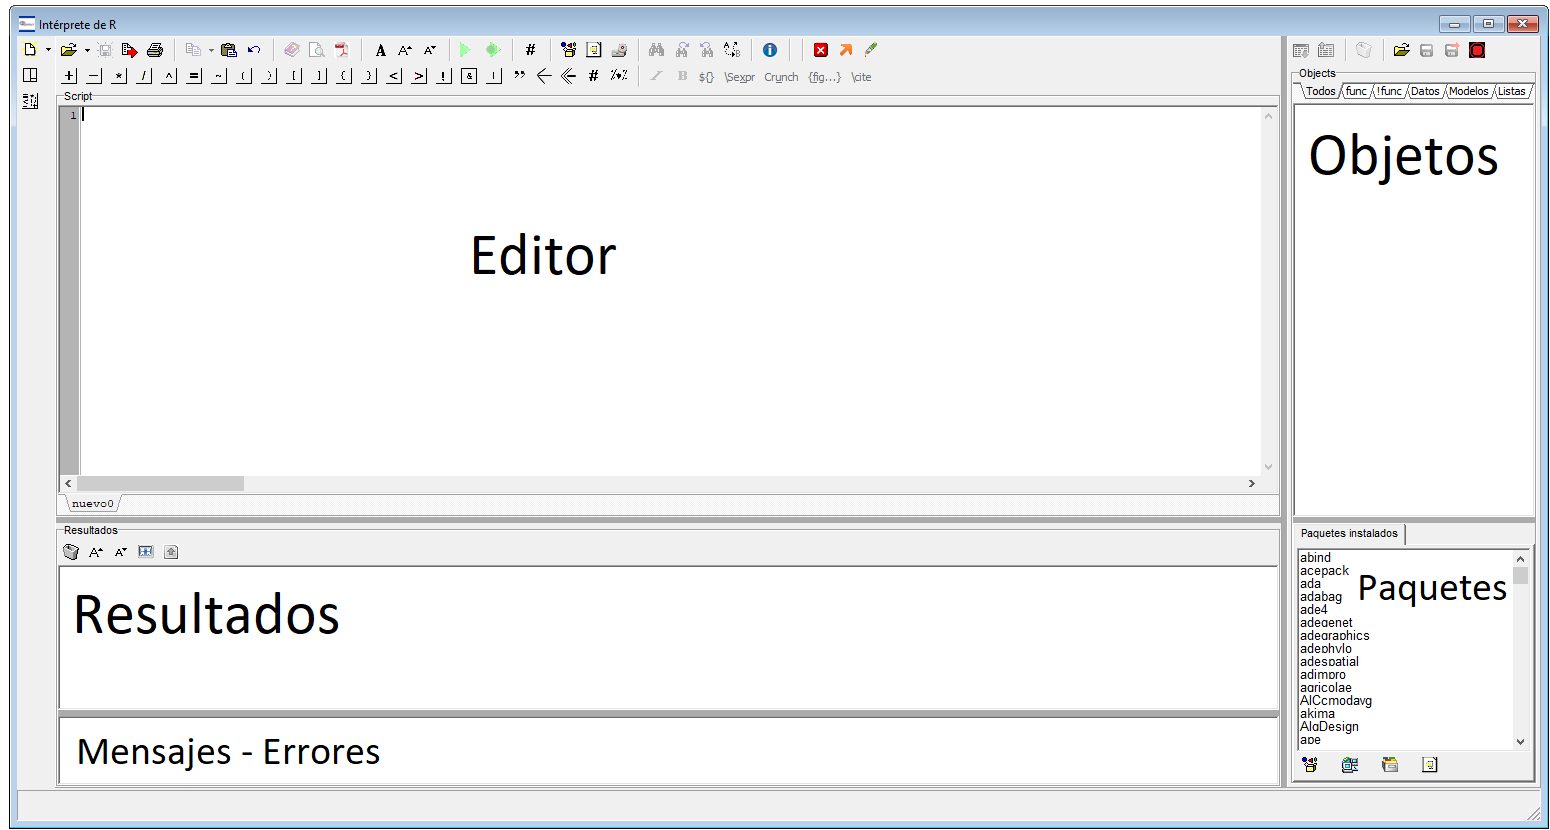
\includegraphics[width=0.8\textwidth,height=\textheight]{images/InfoStatPartes.png}
\caption{Diseño de los paneles del intérprete de R de InfoStat RStudio}
\end{figure}

El panel superior izquierdo permite al usuario visualizar scripts
previamente escritos o escribir nuevos. En el panel inferior izquierdo
se muestran los resultados. En los paneles derechos se muestran los
objetos cargados en el ambiente de trabajo, mientras que en el panel
inferior derecho se muestran los paquetes instalados y en rojo los
paquetes cargados.

\hypertarget{breve-introduccion-a-la-interfaz-de-rstudio}{%
\section{Breve introducción a la interfaz de
RStudio}\label{breve-introduccion-a-la-interfaz-de-rstudio}}

Links de descarga:

\begin{itemize}
\tightlist
\item
  \href{https://www.rstudio.com/products/rstudio/download/\#download}{RStudio}
\end{itemize}

La interfaz de RStudio se divide en cuatro paneles.

\begin{figure}
\centering
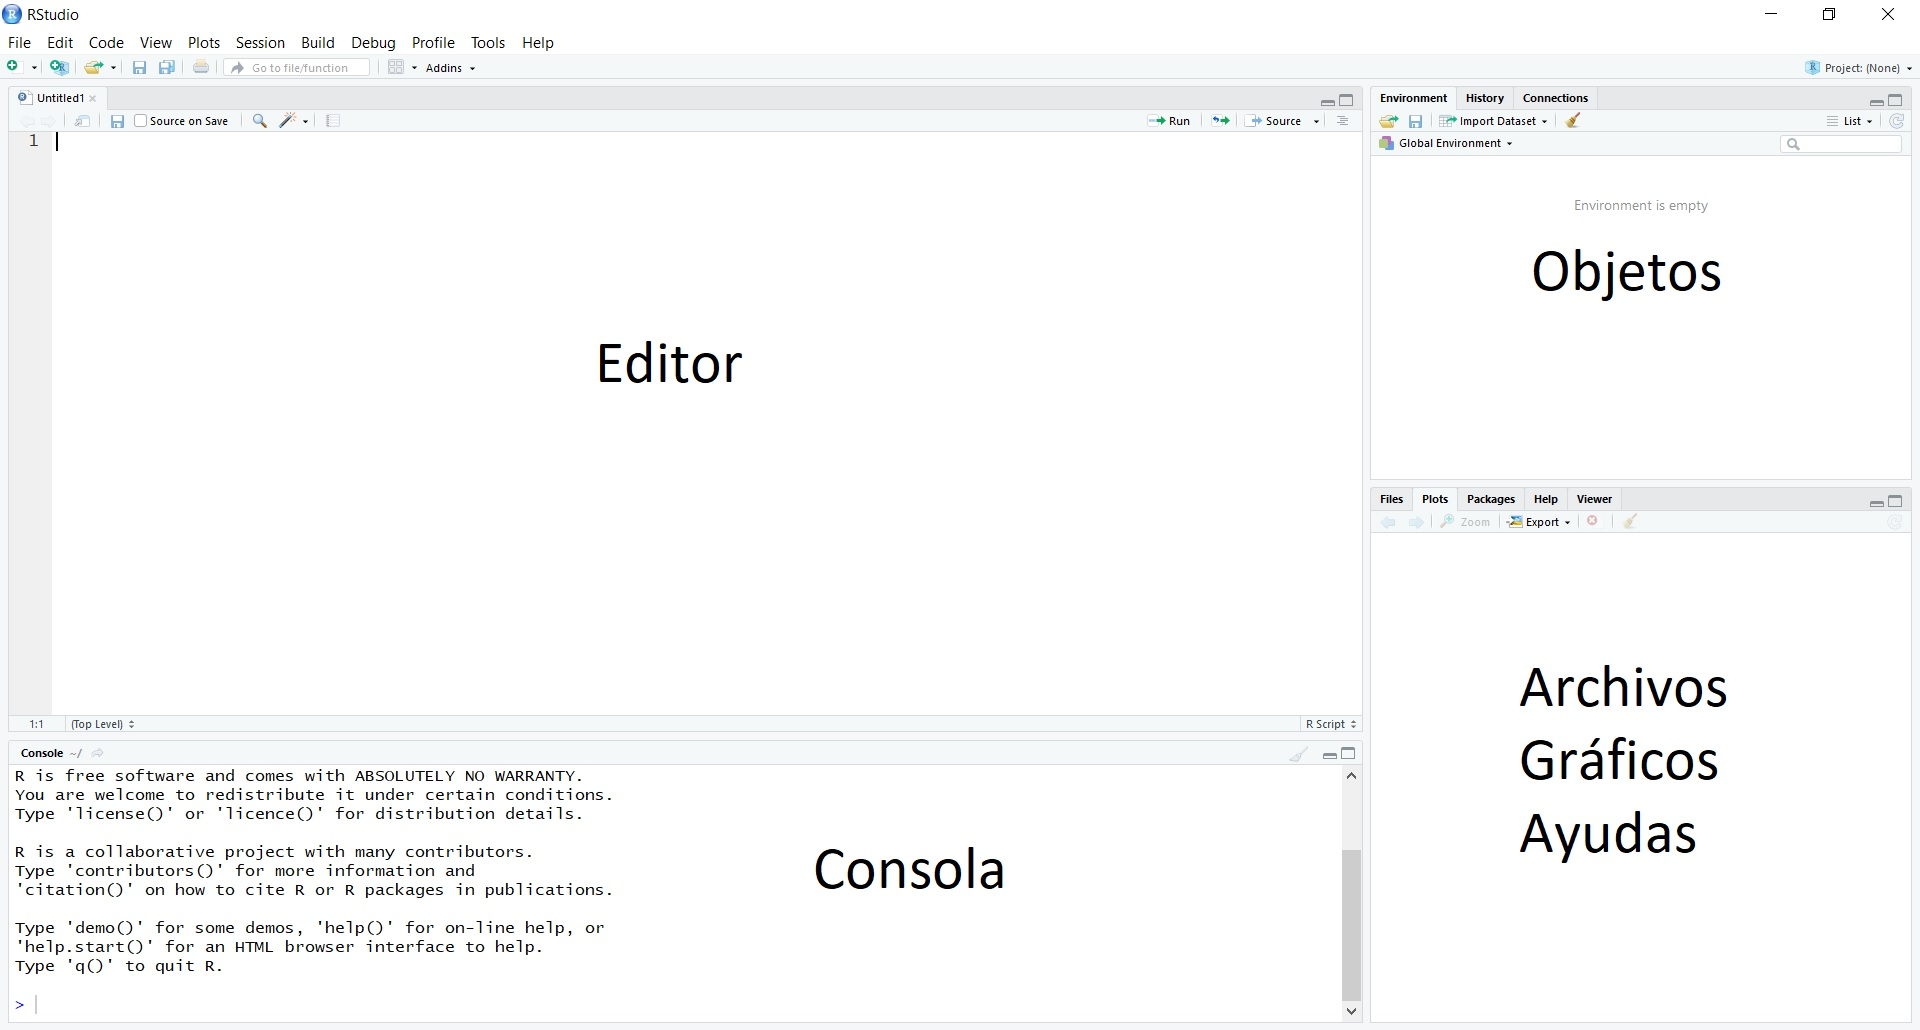
\includegraphics[width=0.8\textwidth,height=\textheight]{images/Rstudiopartes.jpg}
\caption{Diseño de los paneles de RStudio}
\end{figure}

El panel superior izquierdo permite al usuario cargar scripts
previamente escritos o escribir nuevos. En el panel \emph{consola} se
muestran las sentencias de código ejecutadas y los resultados. En los
paneles derechos se muestran los objetos cargados en el ambiente de
trabajo, mientras que en el panel inferior derecho se muestran archivos
en el directorio de trabajo, gráficos generados, ayudas.

\hypertarget{intro}{%
\chapter{Breve introducción a R}\label{intro}}

R \citep{R-base} es un lenguaje de programación orientado a objetos. Fue
creado por Ross Ihaka y Robert Gentleman en 1993 como un dialecto del
software S, fue publicado en 1996 \citep{ihaka1996r}. Es un software
libre y de código abierto, lo que significa que se puede usar, compartir
y modificar el software libremente. Junto con el instalador de R, se
distribuyen ciertos paquetes (\emph{packages}) los cuales incluyen
funciones para implementar algunos métodos estadísticos clásicos y
modernos. Muchas personas utilizan R para realizar análisis estadísticos
por esta razón. Muchos algoritmos y metodologías estadísticas están
disponibles para ser implementadas en R, pero se debe buscar en cual
paquete está disponible y descargarlo para su utilización.

\hypertarget{SintaxisBasica}{%
\section{Generalidades del ambiente R}\label{SintaxisBasica}}

R distingue mayúsculas y minúsculas, esto significa que \texttt{P} y
\texttt{p} son objetos diferentes. Los comandos elementales consisten en
expresiones o asignaciones. Si se ejecuta una expresión el resultado se
imprimirá en la consola pero no se guardará dicho valor. Cuando se
asigna un valor de una expresión (mediante el comando
\texttt{\textless{}-}), el resultado no se imprimirá en pantalla y se
almacenará en un objeto. Comandos diferentes son separados por
\texttt{;} o por una nueva línea. Un conjunto de comandos pueden estar
encerrados entre llaves (\texttt{\{} y \texttt{\}}). Los \texttt{\#}
indican comentarios en el código, todo lo que está a la derecha de este
símbolo no será ejecutado por R. Si se desean hacer comentarios en más
de una línea, cada una de ellas debe comenzar con \#.

Si deseamos guardar en el objeto llamado \texttt{x} el valor de la raíz
cuadrada de 10, debemos utilizar la función \texttt{\textless{}-}:

\begin{Shaded}
\begin{Highlighting}[]
\NormalTok{x <-}\StringTok{ }\KeywordTok{sqrt}\NormalTok{(}\DecValTok{10}\NormalTok{) }\CommentTok{#No se muestra el resultado}
\end{Highlighting}
\end{Shaded}

Para ver el valor de cualquier objeto, se puede especificar el nombre y
ejecutar la línea, por ejemplo si deseamos ver el valor que está
almacenado en \texttt{x} debemos escribir y ejecutar:

\begin{Shaded}
\begin{Highlighting}[]
\NormalTok{x }\CommentTok{#Se muestra el resultado}
\end{Highlighting}
\end{Shaded}

\begin{verbatim}
## [1] 3.162278
\end{verbatim}

\begin{Shaded}
\begin{Highlighting}[]
\KeywordTok{sqrt}\NormalTok{(}\DecValTok{10}\NormalTok{) }\CommentTok{#Se imprime en la consola el resultado}
\end{Highlighting}
\end{Shaded}

\begin{verbatim}
## [1] 3.162278
\end{verbatim}

Las funciones son segmentos de código escrito para llevar a cabo una
tarea específica, en el ejemplo anterior se utilizó la función
\texttt{sqrt} para calcular la raíz cuadrada de 10. Las funciones pueden
necesitar argumentos y devolvuelven uno o más valores en el resultado,
algunas funciones pueden no devolver ningún resultado visible. Los
argumentos de la función son los \emph{inputs} para ejecutar la tarea.
Argumentos deben ir dentro de paréntesis luego del nombre de la función,
cada argumento se separa con \texttt{,} (\texttt{(arg1,arg2\ )}).
Nombres de los argumentos pueden especificarse explicitamente o no. Si
no se detalla el nombre del argumento, R entenderá que están en el mismo
orden que se especificaron cuando se creó la función. En el caso de
\texttt{sqrt} el primer y único argumento de la función es un objeto
numerico.

\begin{rmdnote}
Notar que la mayoría de las funciones de R derivan del inglés y que
utiliza \texttt{.} como separador decimal.
\end{rmdnote}

\#\#Funciones y comandos básicos

En R se puede ejecutar cualquier operación matemática. Comencemos viendo
algunas operaciones básicas:

Suma:

\begin{Shaded}
\begin{Highlighting}[]
\DecValTok{5}\OperatorTok{+}\DecValTok{2}
\end{Highlighting}
\end{Shaded}

\begin{verbatim}
## [1] 7
\end{verbatim}

Raíz cuadrada:

\begin{Shaded}
\begin{Highlighting}[]
\KeywordTok{sqrt}\NormalTok{(}\DecValTok{15}\NormalTok{)}
\end{Highlighting}
\end{Shaded}

\begin{verbatim}
## [1] 3.872983
\end{verbatim}

\hypertarget{tablas_resumen}{%
\subsection{Tablas resumen de operadores y
funciones}\label{tablas_resumen}}

\begin{longtable}[t]{ll}
\caption{\label{tab:funcbasic}Algunas funciones matemáticas en R}\\
\toprule
Sintaxis & Operación\\
\midrule
`x + y` & suma de x e y\\
`x - y` & diferencia de x e y\\
`x * y` & multiplicación de x e y\\
`x / y` & división de x por y\\
`x \%/\% y` & parte entera de la división de x por y\\
\addlinespace
`x \%\% y` & resto de la división de x por y\\
`x \textasciicircum{} y` & x elevado a y-ésima potencia\\
`x < y` & x menor que y\\
`x <= y` & x menor o igual que y\\
`x > y` & x mayor que y\\
\addlinespace
`x >= y` & x mayor o igual que y\\
`x == y` & x igual a y\\
`x != y` & x no es igual a y\\
`sqrt(x)` & raíz cuadrada de x\\
`exp(x)` & exponencial de x\\
\addlinespace
`log(x)` & logaritmo natural de x\\
`log(x, k)` & logaritmo base k de x\\
`sum(x)` & suma de los elementos de x\\
`prod(x)` & producto de los elementos de x\\
`round(x, k)` & x redondeado a k dígitos\\
\bottomrule
\end{longtable}

\hypertarget{ayuda}{%
\subsection{Ayuda}\label{ayuda}}

R incluye documentación de ayuda muy detallada. Para acceder a la ayuda
de cada función, objeto o datos de prueba se debe ejecutar el comando
\texttt{help()} o \texttt{?}. Por ejemplo \texttt{help(sqrt)}, o
\texttt{?sqrt}. Otra forma de pedir la ayuda es presionando F1 luego de
seleccionar la función. La sentencia \texttt{??} busca un patrón dentro
de la documentación del sistema de ayuda, es útil si no se conoce cual
función ejecuta cierto análisis. Otra herramienta muy útil para buscar
ayuda es Google o \href{https://stackoverflow.com/}{Stack Overflow}.

\begin{Shaded}
\begin{Highlighting}[]
\KeywordTok{help}\NormalTok{(sqrt)}
\NormalTok{??square}
\end{Highlighting}
\end{Shaded}

\hypertarget{asignaciones}{%
\subsection{Asignaciones}\label{asignaciones}}

Como ya se especificó en la sección \ref{SintaxisBasica}, un comando de
asignación es \texttt{\textless{}-}, donde a la izquierda se especifica
el nombre del objeto y a la derecha el valor, ya sean resultados de un
cálculo o de un análisis estadístico. Por ejemplo, si se desea asignar
el valor de \texttt{5} al objeto \texttt{radio} se debe ejecutar
\texttt{radio\ \textless{}-\ 5}. Otras formas de hacer asignaciones es
mediante la utilización de \texttt{=} o \texttt{-\textgreater{}}, este
último no es utilizado comúnmente.

Asignaremos al objeto \texttt{x} una secuencia numérica del 1 al 5 y
luego ver el contenido de \texttt{x}:

\begin{Shaded}
\begin{Highlighting}[]
\NormalTok{x<-}\KeywordTok{c}\NormalTok{(}\DecValTok{1}\NormalTok{,}\DecValTok{2}\NormalTok{,}\DecValTok{3}\NormalTok{,}\DecValTok{4}\NormalTok{,}\DecValTok{5}\NormalTok{)  }\CommentTok{#No se muestra el resultado}
\NormalTok{x                }\CommentTok{#Se auto imprime el resultado}
\NormalTok{## [1] 1 2 3 4 5}
\KeywordTok{print}\NormalTok{(x)         }\CommentTok{#Imprime el resultado de manera explícita mediante el comando print }
\NormalTok{## [1] 1 2 3 4 5}
\end{Highlighting}
\end{Shaded}

Otra formas de asignar valores es utilizando \texttt{-\textgreater{}} o
\texttt{=}

\begin{Shaded}
\begin{Highlighting}[]
\KeywordTok{c}\NormalTok{(}\DecValTok{1}\NormalTok{,}\DecValTok{2}\NormalTok{,}\DecValTok{3}\NormalTok{)->x}
\NormalTok{x}
\end{Highlighting}
\end{Shaded}

\begin{verbatim}
## [1] 1 2 3
\end{verbatim}

\begin{Shaded}
\begin{Highlighting}[]
\NormalTok{x=}\KeywordTok{c}\NormalTok{(}\DecValTok{1}\NormalTok{,}\DecValTok{2}\NormalTok{,}\DecValTok{3}\NormalTok{,}\DecValTok{4}\NormalTok{)}
\NormalTok{x}
\end{Highlighting}
\end{Shaded}

\begin{verbatim}
## [1] 1 2 3 4
\end{verbatim}

\begin{rmdnote}
Al utilizar el comando de asignación con el mismo nombre de objeto
(\texttt{x}), cada vez que se utilizó ese comando, el valor que contenía
previamente se reasignó con el valor nuevo.
\end{rmdnote}

\hypertarget{r-como-herramienta-estadistica}{%
\subsection{R como herramienta
estadística}\label{r-como-herramienta-estadistica}}

En el paquete \texttt{stats} (uno de los paquetes instalados por
defecto) permite entre otras cosas, obtener la densidad, función de
distribución (probabilidades), cuantiles y generar números aleatorios de
las distribuciones estadísticas más comunes. Por ejemplo, si se desea
generar 40 números aleatorios de una distribución normal estándar se
deberá ejecutar la sentencia \texttt{rnorm(40)}.

Si se desea calcular medidas descriptivas básicas de un vector se puede
ejecutar \texttt{mean} para calcular la media, \texttt{sd} para calcular
el desvío estándar y \texttt{var} para la varianza. Otra función útil
para obtener valores de posición es la función \texttt{summary}.

\begin{Shaded}
\begin{Highlighting}[]
\NormalTok{x<-}\StringTok{ }\KeywordTok{rnorm}\NormalTok{(}\DecValTok{40}\NormalTok{)}
\KeywordTok{summary}\NormalTok{(x)}
\end{Highlighting}
\end{Shaded}

\begin{verbatim}
##     Min.  1st Qu.   Median     Mean  3rd Qu.     Max. 
## -1.66647 -0.74200 -0.02098 -0.05684  0.72991  1.30036
\end{verbatim}

\hypertarget{r-como-herramienta-grafica}{%
\subsection{R como herramienta
gráfica}\label{r-como-herramienta-grafica}}

Con R se puede realizar gráficos y modificar numerosos parámetros del
gráfico para su publicación. Se realizará un histograma y un boxplot de
la variable \texttt{x} generada anteriormente.

\begin{Shaded}
\begin{Highlighting}[]
\KeywordTok{hist}\NormalTok{(x)}
\end{Highlighting}
\end{Shaded}

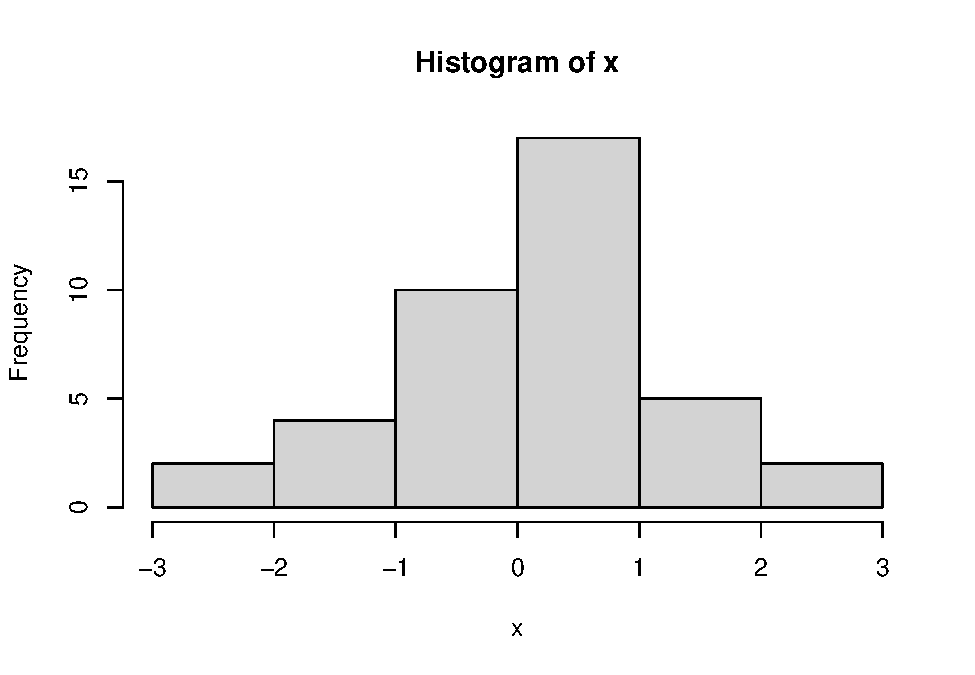
\includegraphics{TutorialR_files/figure-latex/unnamed-chunk-13-1.pdf}

\begin{Shaded}
\begin{Highlighting}[]
\KeywordTok{boxplot}\NormalTok{(x)}
\end{Highlighting}
\end{Shaded}

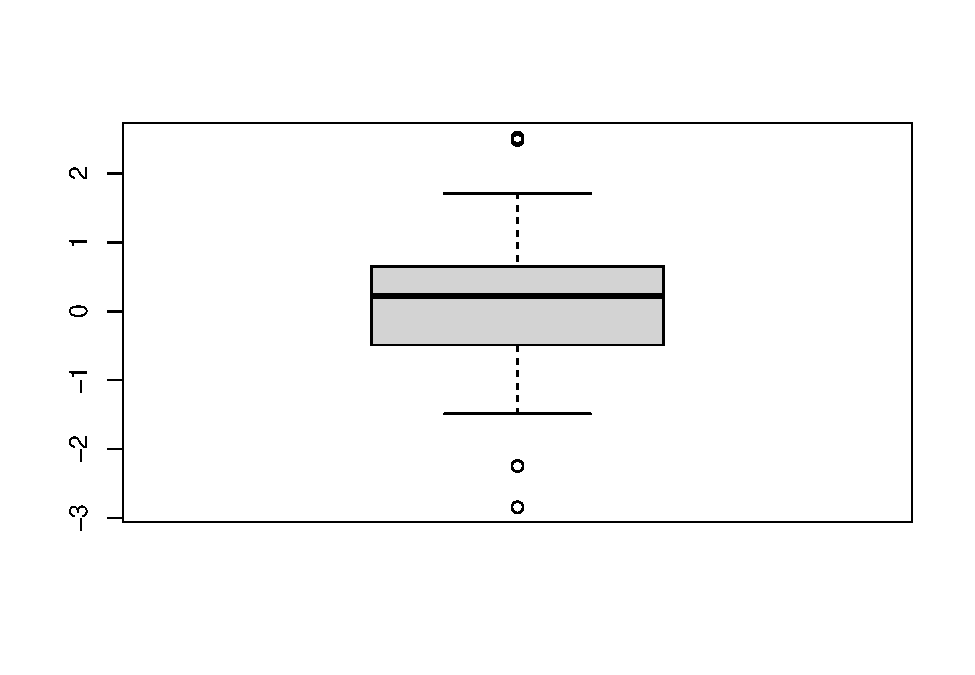
\includegraphics{TutorialR_files/figure-latex/unnamed-chunk-13-2.pdf}

Podría decirse que la función más importante para generar gráficos es
\texttt{plot}. Permite entre otros, realizar diagramas de dispersión y
editar algunos elementos del gráfico.

\begin{Shaded}
\begin{Highlighting}[]
\NormalTok{x <-}\StringTok{ }\KeywordTok{c}\NormalTok{(}\OperatorTok{-}\DecValTok{4}\NormalTok{,}\OperatorTok{-}\DecValTok{3}\NormalTok{,}\OperatorTok{-}\DecValTok{2}\NormalTok{,}\OperatorTok{-}\DecValTok{1}\NormalTok{,}\DecValTok{0}\NormalTok{,}\DecValTok{1}\NormalTok{,}\DecValTok{2}\NormalTok{,}\DecValTok{3}\NormalTok{,}\DecValTok{4}\NormalTok{)  }\CommentTok{# Observar que se remplazó el objeto "x" que se generó previamente}
\NormalTok{y <-}\StringTok{ }\NormalTok{x}\OperatorTok{^}\DecValTok{2}
\KeywordTok{plot}\NormalTok{(x,y)}
\end{Highlighting}
\end{Shaded}

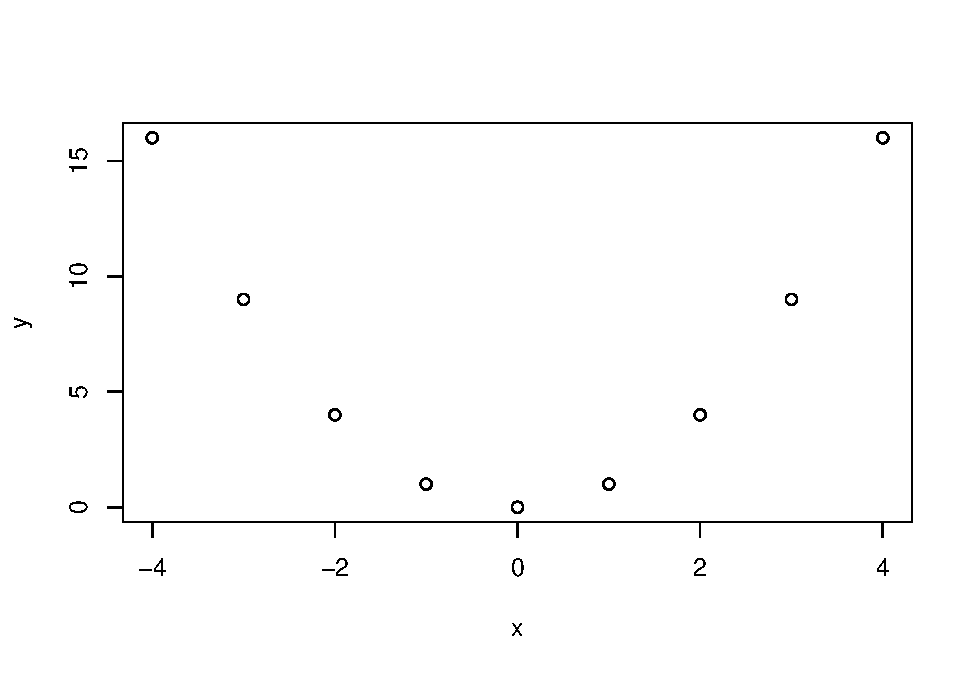
\includegraphics{TutorialR_files/figure-latex/unnamed-chunk-14-1.pdf}

\begin{Shaded}
\begin{Highlighting}[]
\KeywordTok{plot}\NormalTok{(x,y, }\DataTypeTok{type=}\StringTok{"b"}\NormalTok{, }\DataTypeTok{col=}\StringTok{"red"}\NormalTok{)}
\end{Highlighting}
\end{Shaded}

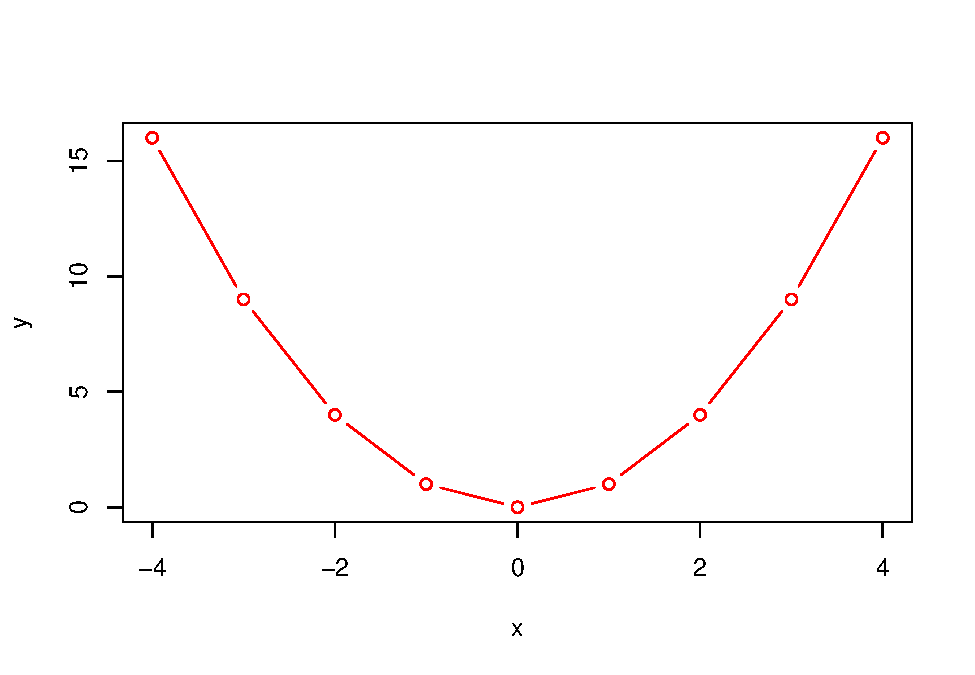
\includegraphics{TutorialR_files/figure-latex/unnamed-chunk-14-2.pdf}

\begin{center}\rule{0.5\linewidth}{\linethickness}\end{center}

\begin{rmdtip}
\hypertarget{ejercitacion}{%
\subsubsection{Ejercitación}\label{ejercitacion}}
\end{rmdtip}

\begin{boxeda}
\begin{enumerate}
\def\labelenumi{\arabic{enumi}.}
\item
  Funciones y comandos básicos

  Calcule la raiz cuadrada de 10

  Calcule el perimetro del círculo de radio 5 (\(P = 2\pi \times r\))

  Calcule 270 dividido la suma entre 12 y 78

  Calcule el cuadrado de 8

  Calcule el logaritmo de 10
\item
  Asignaciones y aritmética vectorial

  Calcule el perímetro del círculo de radio 5 y guárdelo en el objeto
  \texttt{per}.

  Crear el vector de coordenadas 6,7,8,9,10 y llamarlo \texttt{z}Suma de
  dos vectores

  Calcular la suma de \texttt{z} y \texttt{x}

  Calcular el doble de \texttt{x}

  ¿Qué se obtiene haciendo el producto entre los vectores \texttt{z} y
  \texttt{x}?
\item
  R como herramienta estadística

  Generar un vector \texttt{y} con 20 realizaciones de una normal con
  media 5 y desvío estándar 2. Calcular la media y la varianza de
  \texttt{y}. Realizar un histograma.
\end{enumerate}
\end{boxeda}

\hypertarget{objetos-en-r}{%
\chapter{Objetos en R}\label{objetos-en-r}}

Los resultados de un cierto procedimiento o valores pueden ser
almacenados en diferentes clases de objetos. R tiene cinco clases
básicas de objetos, números (\texttt{numeric}), números complejos
(\texttt{complex}), cadenas de caracteres (\texttt{character}), factores
(\texttt{factor}) y valores lógicos (\texttt{logical}). Éstos pueden
juntarse para formar vectores (\texttt{vector}), matrices
(\texttt{matrix}), hojas de datos (\texttt{data.frame}) o listas
(\texttt{list}). Otras clases de objetos pueden ser funciones, modelos,
objetos espaciales, entre otros. En esta sección trabajaremos con
algunos de ellos. Para conocer la clase de un objeto se utiliza la
función \texttt{class}.

\hypertarget{vectores}{%
\section{Vectores}\label{vectores}}

Es el objeto más simple de R. Es importante tener en cuenta que los
vectores solo contienen elementos de la \textbf{misma} clase. La función
\texttt{c()} puede utilizarse para crear vectores concatenando sus
argumentos.

\begin{Shaded}
\begin{Highlighting}[]
\NormalTok{x <-}\StringTok{ }\KeywordTok{c}\NormalTok{(}\DecValTok{2}\NormalTok{,}\DecValTok{4}\NormalTok{,}\DecValTok{6}\NormalTok{)                 }\CommentTok{#numérico (enteros) }
\NormalTok{a <-}\StringTok{ }\KeywordTok{c}\NormalTok{(}\OperatorTok{-}\DecValTok{1}\NormalTok{,}\DecValTok{5}\NormalTok{,}\DecValTok{9}\NormalTok{,}\FloatTok{10.5}\NormalTok{)           }\CommentTok{#numérico (contínuo)}
\NormalTok{d <-}\StringTok{ }\KeywordTok{c}\NormalTok{(}\DecValTok{4}\OperatorTok{+}\NormalTok{2i, }\DecValTok{2}\OperatorTok{+}\NormalTok{5i)            }\CommentTok{#números complejos}
\NormalTok{y <-}\StringTok{ }\KeywordTok{c}\NormalTok{(}\StringTok{"a"}\NormalTok{, }\StringTok{"b"}\NormalTok{, }\StringTok{"c"}\NormalTok{)         }\CommentTok{#caracteres}
\NormalTok{z <-}\StringTok{ }\KeywordTok{c}\NormalTok{(}\OtherTok{TRUE}\NormalTok{, }\OtherTok{TRUE}\NormalTok{, }\OtherTok{FALSE}\NormalTok{, T)  }\CommentTok{#lógico}
\end{Highlighting}
\end{Shaded}

Si quisieramos concatenar \texttt{x} y \texttt{a} podemos llamar esos
objetos dentro de la función \texttt{c()}. Para calcular la longitud del
objeto se utiliza la función \texttt{length()}

\begin{Shaded}
\begin{Highlighting}[]
\NormalTok{x <-}\StringTok{ }\KeywordTok{c}\NormalTok{(}\DecValTok{2}\NormalTok{,}\DecValTok{4}\NormalTok{,}\DecValTok{6}\NormalTok{)             }
\NormalTok{a <-}\StringTok{ }\KeywordTok{c}\NormalTok{(}\OperatorTok{-}\DecValTok{1}\NormalTok{,}\DecValTok{5}\NormalTok{,}\DecValTok{9}\NormalTok{,}\FloatTok{10.5}\NormalTok{)       }
\NormalTok{x_a <-}\StringTok{ }\KeywordTok{c}\NormalTok{(x,a)}
\NormalTok{x_a}
\NormalTok{## [1]  2.0  4.0  6.0 -1.0  5.0  9.0 10.5}
\KeywordTok{length}\NormalTok{(x_a)}
\NormalTok{## [1] 7}
\end{Highlighting}
\end{Shaded}

\begin{rmdnote}
Note que en el ejemplo anterior \texttt{T} y \texttt{F} es la forma
corta de especificar \texttt{TRUE} y \texttt{FALSE}. Es recomendable
utilizar la forma explícita de \texttt{TRUE} y \texttt{FALSE} que la
forma corta, dado que \texttt{T} y \texttt{F} son símbolos que pueden
redefinirse, por lo que no se debería asumir que siempre se van a
evaluar como operadores lógicos.
\end{rmdnote}

\hypertarget{secuencias}{%
\subsection{Secuencias}\label{secuencias}}

\begin{Shaded}
\begin{Highlighting}[]
\NormalTok{x <-}\StringTok{ }\KeywordTok{c}\NormalTok{(}\DecValTok{1}\NormalTok{, }\DecValTok{2}\NormalTok{, }\DecValTok{3}\NormalTok{, }\DecValTok{4}\NormalTok{, }\DecValTok{5}\NormalTok{) }
\NormalTok{x <-}\StringTok{ }\DecValTok{1}\OperatorTok{:}\DecValTok{10}
\NormalTok{y <-}\StringTok{ }\DecValTok{-5}\OperatorTok{:}\DecValTok{3}
\end{Highlighting}
\end{Shaded}

Para generar secuencias de números enteros consecutivos se puede
utilizar \texttt{:}, pero si se desea generar otros tipos de secuencias,
por ejemplo la secuencia 4,6,8,\ldots{},20, se debe utilizar la función
\texttt{seq}.

\begin{Shaded}
\begin{Highlighting}[]
\KeywordTok{seq}\NormalTok{(}\DataTypeTok{from =} \DecValTok{4}\NormalTok{, }\DataTypeTok{to =} \DecValTok{20}\NormalTok{, }\DataTypeTok{by =} \DecValTok{2}\NormalTok{)}
\end{Highlighting}
\end{Shaded}

\begin{verbatim}
## [1]  4  6  8 10 12 14 16 18 20
\end{verbatim}

\begin{rmdnote}
Los argumentos de la función \texttt{seq}, permiten generar secuencia,
desde (\texttt{from} y, hasta (\texttt{to}) los valores especificados.
Se pueden especificar el incremento de cada valor (\texttt{by}), o puede
definirse el largo de la secuencia deseada (\texttt{length.out}).
\end{rmdnote}

\hypertarget{vectores-con-valores-repetidos}{%
\subsection{Vectores con valores
repetidos}\label{vectores-con-valores-repetidos}}

Cuando se desea generar un vector con valores repetidos se puede
utilizar la función \texttt{rep}. Esta función replica los valores que
se espicifican en el primer argumento, tantas veces o hasta alcanzar la
longitud total que se especifique.

\begin{Shaded}
\begin{Highlighting}[]
\KeywordTok{rep}\NormalTok{(}\DecValTok{1}\NormalTok{, }\DecValTok{5}\NormalTok{)}
\NormalTok{## [1] 1 1 1 1 1}
\NormalTok{x <-}\StringTok{ }\DecValTok{1}\OperatorTok{:}\DecValTok{3}
\KeywordTok{rep}\NormalTok{(x, }\DecValTok{2}\NormalTok{)}
\NormalTok{## [1] 1 2 3 1 2 3}
\KeywordTok{rep}\NormalTok{(x, }\KeywordTok{c}\NormalTok{(}\DecValTok{2}\NormalTok{,}\DecValTok{4}\NormalTok{,}\DecValTok{1}\NormalTok{)) }\CommentTok{#En este caso repetirá el 1 dos vecesm el 2 cuatro veces y el 3 una vez.}
\NormalTok{## [1] 1 1 2 2 2 2 3}
\KeywordTok{rep}\NormalTok{(x, }\DataTypeTok{length =} \DecValTok{8}\NormalTok{)}
\NormalTok{## [1] 1 2 3 1 2 3 1 2}
\end{Highlighting}
\end{Shaded}

\hypertarget{vectores-de-factores}{%
\subsection{Vectores de factores}\label{vectores-de-factores}}

Los vectores que se generan pueden convertirse en factores, para ello se
utiliza la función \texttt{as.factor}.

\begin{Shaded}
\begin{Highlighting}[]
\NormalTok{x_f <-}\StringTok{ }\KeywordTok{as.factor}\NormalTok{(x)}
\end{Highlighting}
\end{Shaded}

Tambien pueden generarse vectores que contiene factores utilizando
\texttt{gl}. A esta función se le debe especificar el número de niveles
del factor y el número de repeticiones. Se le puede especificar el largo
del vector y las etiquetas (\texttt{labels}) de los factores.

\begin{Shaded}
\begin{Highlighting}[]
\KeywordTok{gl}\NormalTok{(}\DecValTok{3}\NormalTok{, }\DecValTok{5}\NormalTok{)}
\end{Highlighting}
\end{Shaded}

\begin{verbatim}
##  [1] 1 1 1 1 1 2 2 2 2 2 3 3 3 3 3
## Levels: 1 2 3
\end{verbatim}

\begin{Shaded}
\begin{Highlighting}[]
\KeywordTok{gl}\NormalTok{(}\DecValTok{3}\NormalTok{, }\DecValTok{5}\NormalTok{, }\DataTypeTok{length =} \DecValTok{30}\NormalTok{)}
\end{Highlighting}
\end{Shaded}

\begin{verbatim}
##  [1] 1 1 1 1 1 2 2 2 2 2 3 3 3 3 3 1 1 1 1 1 2 2 2 2 2 3 3 3 3 3
## Levels: 1 2 3
\end{verbatim}

\begin{Shaded}
\begin{Highlighting}[]
\KeywordTok{gl}\NormalTok{(}\DecValTok{3}\NormalTok{, }\DecValTok{5}\NormalTok{, }\DataTypeTok{labels =} \KeywordTok{c}\NormalTok{(}\StringTok{"grupo A"}\NormalTok{, }\StringTok{"grupo B"}\NormalTok{, }\StringTok{"grupo C"}\NormalTok{))}
\end{Highlighting}
\end{Shaded}

\begin{verbatim}
##  [1] grupo A grupo A grupo A grupo A grupo A grupo B grupo B grupo B
##  [9] grupo B grupo B grupo C grupo C grupo C grupo C grupo C
## Levels: grupo A grupo B grupo C
\end{verbatim}

\hypertarget{seleccion-de-elementos-de-un-vector}{%
\subsection{Seleccion de elementos de un
vector}\label{seleccion-de-elementos-de-un-vector}}

Los corchetes (\texttt{{[}\ {]}}) se utilizan para indicar posición de
un objeto. Se utilizan del lado derecho del objeto. Dado que los
vectores son elementos de una dimensión, si se desea seleccionar el
primer elemento del objeto \texttt{x} se debe indicar \texttt{x{[}1{]}}.

\begin{Shaded}
\begin{Highlighting}[]
\NormalTok{x <-}\StringTok{ }\KeywordTok{c}\NormalTok{(}\DecValTok{3}\NormalTok{,}\DecValTok{52}\NormalTok{,}\OperatorTok{-}\DecValTok{8}\NormalTok{,}\DecValTok{2}\NormalTok{,}\DecValTok{1}\NormalTok{,}\DecValTok{7}\NormalTok{,}\DecValTok{11}\NormalTok{,}\OperatorTok{-}\DecValTok{3}\NormalTok{,}\DecValTok{0}\NormalTok{,}\DecValTok{6}\NormalTok{,}\DecValTok{23}\NormalTok{,}\DecValTok{17}\NormalTok{)}
\NormalTok{x[}\DecValTok{1}\NormalTok{]}
\end{Highlighting}
\end{Shaded}

\begin{verbatim}
## [1] 3
\end{verbatim}

\begin{Shaded}
\begin{Highlighting}[]
\NormalTok{x[}\DecValTok{3}\NormalTok{]}
\end{Highlighting}
\end{Shaded}

\begin{verbatim}
## [1] -8
\end{verbatim}

\begin{Shaded}
\begin{Highlighting}[]
\NormalTok{x[}\KeywordTok{c}\NormalTok{(}\DecValTok{1}\NormalTok{, }\DecValTok{3}\NormalTok{)]}
\end{Highlighting}
\end{Shaded}

\begin{verbatim}
## [1]  3 -8
\end{verbatim}

Si se desea sustituir un elemento del vector se puede utilizar el signo
de asignación. Por ejemplo, si se desea sustituir el tercer elemento de
x por 88:

\begin{Shaded}
\begin{Highlighting}[]
\NormalTok{x[}\DecValTok{3}\NormalTok{] <-}\StringTok{  }\DecValTok{88}
\NormalTok{x}
\end{Highlighting}
\end{Shaded}

\begin{verbatim}
##  [1]  3 52 88  2  1  7 11 -3  0  6 23 17
\end{verbatim}

Si se quiere obtener un vector sin algunos elementos, se debe anteponer
el signo \texttt{-} al valor del índice.

\begin{Shaded}
\begin{Highlighting}[]
\NormalTok{x[}\OperatorTok{-}\DecValTok{3}\NormalTok{]}
\end{Highlighting}
\end{Shaded}

\begin{verbatim}
##  [1]  3 52  2  1  7 11 -3  0  6 23 17
\end{verbatim}

\hypertarget{matrices}{%
\section{Matrices}\label{matrices}}

Las matrices son vectores con atributo de dimensión (2 dimensiones:
filas y columnas). A diferencia de los \texttt{data.frame}s, todas las
columnas de las matrices son de una misma clase. Para generar matrices
se puede utilizar la función \texttt{matrix}.

\begin{Shaded}
\begin{Highlighting}[]
\NormalTok{x <-}\StringTok{ }\DecValTok{1}\OperatorTok{:}\DecValTok{20}
\KeywordTok{matrix}\NormalTok{(x, }\DataTypeTok{nrow =} \DecValTok{5}\NormalTok{, }\DataTypeTok{ncol =} \DecValTok{4}\NormalTok{)}
\end{Highlighting}
\end{Shaded}

\begin{verbatim}
##      [,1] [,2] [,3] [,4]
## [1,]    1    6   11   16
## [2,]    2    7   12   17
## [3,]    3    8   13   18
## [4,]    4    9   14   19
## [5,]    5   10   15   20
\end{verbatim}

Las matrices pueden ser creadas uniendo filas o columnas mediante las
funciones \texttt{cbind()} y \texttt{rbind()}.

\begin{Shaded}
\begin{Highlighting}[]
\NormalTok{x <-}\StringTok{ }\DecValTok{1}\OperatorTok{:}\DecValTok{3}
\NormalTok{y <-}\StringTok{ }\DecValTok{10}\OperatorTok{:}\DecValTok{12}
\KeywordTok{cbind}\NormalTok{(x, y)}
\end{Highlighting}
\end{Shaded}

\begin{verbatim}
##      x  y
## [1,] 1 10
## [2,] 2 11
## [3,] 3 12
\end{verbatim}

\begin{Shaded}
\begin{Highlighting}[]
\KeywordTok{rbind}\NormalTok{(x, y) }
\end{Highlighting}
\end{Shaded}

\begin{verbatim}
##   [,1] [,2] [,3]
## x    1    2    3
## y   10   11   12
\end{verbatim}

\hypertarget{operaciones-con-matrices}{%
\subsection{Operaciones con matrices:}\label{operaciones-con-matrices}}

\begin{itemize}
\tightlist
\item
  \texttt{A\ \%*\%\ B} : producto de matrices
\item
  \texttt{t(A)} : traspuesta de la matriz A
\item
  \texttt{solve(A)} : inversa de la matriz A
\item
  \texttt{solve(A,b)} : solución del sistema de ecuaciones Ax=b.
\item
  \texttt{svd(A)} : descomposición en valores singulares
\item
  \texttt{qr(A)} : descomposición QR
\item
  \texttt{eigen(A)} : valores y vectores propios
\item
  \texttt{diag(b)} : matriz diagonal. (b es un vector)
\item
  \texttt{diag(A)} : matriz diagonal. (A es una matriz)
\item
  \texttt{A\ \%o\%\ B\ ==\ outer(A,B)} : producto exterior de dos
  vectores o matrices
\end{itemize}

\hypertarget{listas}{%
\section{Listas}\label{listas}}

Una lista es la forma generalizada de un vector que puede contener
elementos de diferentes clases (número, vector, matriz, lista, etc.).
Para crear lista se puede utilizar la función \texttt{list()}. Dada su
flexibilidad son contenedores generales de datos. Muchas funciones
devuelven un conjunto de resultados de distinta longitud y distinto tipo
en forma de lista.

\begin{Shaded}
\begin{Highlighting}[]
\NormalTok{n <-}\StringTok{  }\KeywordTok{c}\NormalTok{(}\DecValTok{2}\NormalTok{, }\DecValTok{4}\NormalTok{, }\DecValTok{6}\NormalTok{)}
\NormalTok{s <-}\StringTok{  }\KeywordTok{c}\NormalTok{(}\StringTok{"aa"}\NormalTok{, }\StringTok{"bb"}\NormalTok{, }\StringTok{"cc"}\NormalTok{, }\StringTok{"dd"}\NormalTok{, }\StringTok{"ee"}\NormalTok{)}
\NormalTok{b <-}\StringTok{  }\KeywordTok{c}\NormalTok{(}\OtherTok{TRUE}\NormalTok{, }\OtherTok{FALSE}\NormalTok{, }\OtherTok{TRUE}\NormalTok{, }\OtherTok{FALSE}\NormalTok{, }\OtherTok{FALSE}\NormalTok{)}
\NormalTok{x <-}\StringTok{  }\KeywordTok{list}\NormalTok{(n, s, b)}
\NormalTok{x}
\end{Highlighting}
\end{Shaded}

\begin{verbatim}
## [[1]]
## [1] 2 4 6
## 
## [[2]]
## [1] "aa" "bb" "cc" "dd" "ee"
## 
## [[3]]
## [1]  TRUE FALSE  TRUE FALSE FALSE
\end{verbatim}

\hypertarget{hojas-de-datos-data-frames}{%
\section{Hojas de datos (Data
frames)}\label{hojas-de-datos-data-frames}}

Es el objeto más común en R para almacenar datos. Sus columnas pueden
ser de diferentes clases por ejemplo variables continuas y categóricas.
Este tipo de objetos puede generarse mediante la función
\texttt{data.frame()}.

\begin{rmdnote}
\texttt{data.frame} convierte los vectores de caracteres en factores
automáticamente.
\end{rmdnote}

\begin{Shaded}
\begin{Highlighting}[]
\NormalTok{x1 <-}\StringTok{ }\DecValTok{1}\OperatorTok{:}\DecValTok{10}
\NormalTok{x2 <-}\StringTok{ }\DecValTok{24}\OperatorTok{:}\DecValTok{33}
\NormalTok{x3 <-}\StringTok{ }\KeywordTok{gl}\NormalTok{(}\DecValTok{2}\NormalTok{, }\DecValTok{5}\NormalTok{, }\DataTypeTok{labels =} \KeywordTok{c}\NormalTok{(}\StringTok{"si"}\NormalTok{,}\StringTok{"no"}\NormalTok{))}
\NormalTok{x4 <-letters[}\DecValTok{1}\OperatorTok{:}\DecValTok{10}\NormalTok{]}
\KeywordTok{data.frame}\NormalTok{(}\DataTypeTok{A =}\NormalTok{ x1, }\DataTypeTok{B =}\NormalTok{ x2, }\DataTypeTok{C =}\NormalTok{ x3, }\DataTypeTok{D =}\NormalTok{ x4)}
\end{Highlighting}
\end{Shaded}

\begin{verbatim}
##     A  B  C D
## 1   1 24 si a
## 2   2 25 si b
## 3   3 26 si c
## 4   4 27 si d
## 5   5 28 si e
## 6   6 29 no f
## 7   7 30 no g
## 8   8 31 no h
## 9   9 32 no i
## 10 10 33 no j
\end{verbatim}

\begin{center}\rule{0.5\linewidth}{\linethickness}\end{center}

\begin{rmdtip}
\hypertarget{ejercitacion}{%
\subsection{Ejercitación}\label{ejercitacion}}
\end{rmdtip}

\begin{boxeda}
\begin{enumerate}
\def\labelenumi{\arabic{enumi}.}
\item
  Vectores

  Genere un vector \texttt{b} el cual contenga los valores de \texttt{x}
  y \texttt{a} ¿Cuantos elementos tiene el vector \texttt{b}?
\item
  Secuencias

  Genere la secuencia 8,7,6,5,4

  seq(4,20,2) ¿Este comando da eror? ¿Por qué?

  Genere usando comandos para secuencias el vector de componentes: 1, 2,
  3, 4, 5, 6, 73, 72, 71, 70, 69, 68, 3, 6, 9, 12, 15, 18.
\item
  Repetir valores

  Genere un vector de componentes ``azul'', ``azul'',``azul'', ``azul'',
  ``amarillo'', ``amarillo'', ``verde'', ``verde'',``verde'', llamado
  \texttt{col}. ¿Es un vector de factores?
\item
  Matrices

  Calcule la inversa y los autovalores y autovectores de
  \texttt{A\ \ =\ \ matrix(c(1,3,3,9,5,9,3,5,6),\ nrow\ =\ 3)}
\end{enumerate}
\end{boxeda}

\hypertarget{control-de-flujo}{%
\chapter{Control de flujo}\label{control-de-flujo}}

\hypertarget{construccion-condicional-if}{%
\section{\texorpdfstring{Construcción condicional
\texttt{if}}{Construcción condicional if}}\label{construccion-condicional-if}}

Es de la forma \texttt{if\ (expr\ 1)\ expr\ 2\ else\ expr\ 3} donde
\texttt{expr\ 1} debe producir un valor logico. Si \texttt{expr\ 1} es
verdadero (\texttt{T}), se ejecutara \texttt{expr\ 2}. Si
\texttt{expr\ 1} es falso (\texttt{F}), y se ha escrito la opcion else,
que es opcional, se ejecutara \texttt{expr\ 3}.

\begin{Shaded}
\begin{Highlighting}[]
\ControlFlowTok{if}\NormalTok{( }\DecValTok{3} \OperatorTok{>}\StringTok{ }\DecValTok{2}\NormalTok{) }\KeywordTok{print}\NormalTok{(}\StringTok{"yes"}\NormalTok{)}
\end{Highlighting}
\end{Shaded}

\begin{verbatim}
## [1] "yes"
\end{verbatim}

\begin{Shaded}
\begin{Highlighting}[]
\ControlFlowTok{if}\NormalTok{( }\DecValTok{2} \OperatorTok{>}\StringTok{ }\DecValTok{3}\NormalTok{) }\KeywordTok{print}\NormalTok{(}\StringTok{"yes"}\NormalTok{)}
\ControlFlowTok{if}\NormalTok{( }\DecValTok{2} \OperatorTok{>}\StringTok{ }\DecValTok{3}\NormalTok{) }\KeywordTok{print}\NormalTok{(}\StringTok{"yes"}\NormalTok{) }\ControlFlowTok{else} \KeywordTok{print}\NormalTok{(}\StringTok{"no"}\NormalTok{)}
\end{Highlighting}
\end{Shaded}

\begin{verbatim}
## [1] "no"
\end{verbatim}

Ejemplo con dos condiciones supongamos que \texttt{x\ \textless{}-\ 75}
es la nota numerica de examen de un alumno, queremos asignar nota ``A'',
``B'' o ``C''

\begin{Shaded}
\begin{Highlighting}[]
\ControlFlowTok{if}\NormalTok{(x }\OperatorTok{<}\StringTok{ }\DecValTok{60}\NormalTok{) nota =}\StringTok{ "C"}
\ControlFlowTok{if}\NormalTok{(x }\OperatorTok{>=}\StringTok{ }\DecValTok{60} \OperatorTok{&}\StringTok{ }\NormalTok{x }\OperatorTok{<}\StringTok{ }\DecValTok{80}\NormalTok{) nota =}\StringTok{ "B"}
\ControlFlowTok{if}\NormalTok{(x }\OperatorTok{>=}\StringTok{  }\DecValTok{80}\NormalTok{) nota =}\StringTok{ "A"}
\end{Highlighting}
\end{Shaded}

\texttt{ifelse} es la versión vectorizada de \texttt{if}

Ejemplo

\begin{Shaded}
\begin{Highlighting}[]
\NormalTok{nota.num <-}\StringTok{ }\KeywordTok{c}\NormalTok{(}\DecValTok{39}\NormalTok{, }\DecValTok{51}\NormalTok{, }\DecValTok{60}\NormalTok{, }\DecValTok{65}\NormalTok{, }\DecValTok{72}\NormalTok{, }\DecValTok{78}\NormalTok{, }\DecValTok{79}\NormalTok{, }\DecValTok{83}\NormalTok{, }\DecValTok{85}\NormalTok{, }\DecValTok{85}\NormalTok{, }\DecValTok{87}\NormalTok{, }\DecValTok{89}\NormalTok{, }\DecValTok{91}\NormalTok{, }\DecValTok{95}\NormalTok{, }\DecValTok{96}\NormalTok{, }\DecValTok{97}\NormalTok{, }\DecValTok{100}\NormalTok{, }\DecValTok{100}\NormalTok{)}

\NormalTok{prueba <-}\StringTok{ }\KeywordTok{ifelse}\NormalTok{ (nota.num }\OperatorTok{>=}\StringTok{ }\DecValTok{60}\NormalTok{, }\StringTok{"aprobado"}\NormalTok{, }\StringTok{"desaprobado"}\NormalTok{)}
\NormalTok{prueba}
\end{Highlighting}
\end{Shaded}

\begin{verbatim}
##  [1] "desaprobado" "desaprobado" "aprobado"    "aprobado"    "aprobado"   
##  [6] "aprobado"    "aprobado"    "aprobado"    "aprobado"    "aprobado"   
## [11] "aprobado"    "aprobado"    "aprobado"    "aprobado"    "aprobado"   
## [16] "aprobado"    "aprobado"    "aprobado"
\end{verbatim}

\hypertarget{construccion-repetitiva-for}{%
\section{\texorpdfstring{Construcción repetitiva
\texttt{for}}{Construcción repetitiva for}}\label{construccion-repetitiva-for}}

Es de la forma \texttt{for\ (nombre\ in\ expr\ 1)\ expr\ 2} donde
\texttt{nombre} es la variable de control de iteración, \texttt{expr\ 1}
es un vector (a menudo de la forma \texttt{m:n}), y \texttt{expr\ 2} es
una expresión, a menudo agrupada, en cuyas sub-expresiones puede
aparecer la variable de control, \texttt{nombre}. \texttt{expr\ 2} se
evalua repetidamente conforme \texttt{nombre} recorre los valores del
vector \texttt{expr\ 1}.

\begin{Shaded}
\begin{Highlighting}[]
\ControlFlowTok{for}\NormalTok{ (i }\ControlFlowTok{in} \DecValTok{1}\OperatorTok{:}\DecValTok{10}\NormalTok{) }\KeywordTok{print}\NormalTok{(i)}
\end{Highlighting}
\end{Shaded}

\begin{verbatim}
## [1] 1
## [1] 2
## [1] 3
## [1] 4
## [1] 5
## [1] 6
## [1] 7
## [1] 8
## [1] 9
## [1] 10
\end{verbatim}

\begin{Shaded}
\begin{Highlighting}[]
\NormalTok{x =}\StringTok{ }\KeywordTok{numeric}\NormalTok{(}\DecValTok{10}\NormalTok{)}
\ControlFlowTok{for}\NormalTok{ (i }\ControlFlowTok{in} \DecValTok{1}\OperatorTok{:}\DecValTok{10}\NormalTok{) x[i] =}\StringTok{ }\NormalTok{i}\OperatorTok{^}\DecValTok{2}

\NormalTok{y =}\StringTok{ }\DecValTok{0}
\ControlFlowTok{for}\NormalTok{ (i }\ControlFlowTok{in} \DecValTok{1}\OperatorTok{:}\DecValTok{10}\NormalTok{) y =}\StringTok{ }\NormalTok{y }\OperatorTok{+}\StringTok{ }\NormalTok{i}
\end{Highlighting}
\end{Shaded}

\hypertarget{construccion-repetitiva-while}{%
\section{\texorpdfstring{Construccion repetitiva
\texttt{while}}{Construccion repetitiva while}}\label{construccion-repetitiva-while}}

Es de la forma \texttt{while\ (expr1)\ expr2}, indicando que se quiere
repetir la acción \texttt{expr2} mientras que ocurra \texttt{expr1}.

\begin{Shaded}
\begin{Highlighting}[]
\NormalTok{i =}\StringTok{ }\DecValTok{0}
\ControlFlowTok{while}\NormalTok{ (i }\OperatorTok{<}\StringTok{ }\DecValTok{15}\NormalTok{) \{}\KeywordTok{print}\NormalTok{(i); i =}\StringTok{ }\NormalTok{i}\OperatorTok{+}\DecValTok{1}\NormalTok{\}}
\end{Highlighting}
\end{Shaded}

\begin{verbatim}
## [1] 0
## [1] 1
## [1] 2
## [1] 3
## [1] 4
## [1] 5
## [1] 6
## [1] 7
## [1] 8
## [1] 9
## [1] 10
## [1] 11
## [1] 12
## [1] 13
## [1] 14
\end{verbatim}

\begin{center}\rule{0.5\linewidth}{\linethickness}\end{center}

\begin{rmdtip}
\hypertarget{ejercitacion}{%
\subsection{Ejercitación}\label{ejercitacion}}
\end{rmdtip}

\begin{boxeda}
\begin{enumerate}
\def\labelenumi{\arabic{enumi}.}
\item
  Construcción condicional

  Si se quiere poner notas ``A'', ``B'' o ``C'': ``C'' si final\_score
  \textless{}60, ``B'' si 60 =\textless{} final\_score \textless{} 80,
  ``A'' si 80 =\textless{} final\_score =\textless{} 100.
\item
  Construcción repetitiva

  Usar un ciclo \texttt{for} para contar la cantidad de números mayores
  a 10 en el vector
  \texttt{x\ \textless{}-\ c(2,5,3,9,8,11,6,8,12,3,57,56)}
\end{enumerate}
\end{boxeda}

\hypertarget{generar-nuevas-funciones}{%
\chapter{Generar nuevas funciones}\label{generar-nuevas-funciones}}

R es un lenguaje que permite crear nuevas funciones. Una funcion se
define con una asignacion de la forma:

\begin{Shaded}
\begin{Highlighting}[]
\NormalTok{nombre <-}\StringTok{ }\ControlFlowTok{function}\NormalTok{(arg1, arg2, ...) \{}
\NormalTok{   expresion}
\NormalTok{ \}}
\end{Highlighting}
\end{Shaded}

La \texttt{expresion} es una fórmula o grupo de formulas (o sentencias)
que utilizan los argumentos para calcular uno o varios valores. El
resultado de dicha expresión es el valor que proporciona R en su salida
y este puede ser un número, un vector, un gráfico, una lista y/o un
mensaje. Una función devuelve el último valor impreso en la consola.

Ejemplos:

\begin{Shaded}
\begin{Highlighting}[]
\NormalTok{funcion1 <-}\StringTok{ }\ControlFlowTok{function}\NormalTok{(x)\{ y =}\StringTok{ }\NormalTok{x }\OperatorTok{+}\StringTok{ }\DecValTok{4}\NormalTok{\}}

\NormalTok{(a<-}\KeywordTok{funcion1}\NormalTok{(}\DecValTok{5}\NormalTok{))}
\end{Highlighting}
\end{Shaded}

\begin{verbatim}
## [1] 9
\end{verbatim}

En en caso siguiente, si se desea guardar el resultado en un objeto solo
se guardará el rango (último valor impreso en consola).

\begin{Shaded}
\begin{Highlighting}[]
\NormalTok{funcion2 <-}\StringTok{ }\ControlFlowTok{function}\NormalTok{(muestra)\{     }\CommentTok{#El único argumento es un vector de datos}
\NormalTok{  media =}\StringTok{ }\KeywordTok{mean}\NormalTok{(muestra, }\DataTypeTok{na.rm =}\NormalTok{ T)}
\NormalTok{  varianza =}\StringTok{ }\KeywordTok{var}\NormalTok{(muestra, }\DataTypeTok{na.rm =}\NormalTok{ T)}
\NormalTok{  rango =}\StringTok{ }\KeywordTok{max}\NormalTok{(muestra, }\DataTypeTok{na.rm =}\NormalTok{ T) }\OperatorTok{-}\StringTok{ }\KeywordTok{min}\NormalTok{(muestra, }\DataTypeTok{na.rm =}\NormalTok{ T)}
  \KeywordTok{print}\NormalTok{(media)}
  \KeywordTok{print}\NormalTok{(varianza)}
  \KeywordTok{print}\NormalTok{(rango)}

\NormalTok{\}}

\KeywordTok{funcion2}\NormalTok{(}\KeywordTok{rnorm}\NormalTok{(}\DecValTok{40}\NormalTok{,}\DecValTok{5}\NormalTok{,}\DecValTok{16}\NormalTok{))}
\end{Highlighting}
\end{Shaded}

\begin{verbatim}
## [1] 5.603092
## [1] 216.2479
## [1] 63.42857
\end{verbatim}

Para que guarde los tres resultados hay que especificar que se haga una
lista o vector.

\begin{Shaded}
\begin{Highlighting}[]
\NormalTok{funcion3 <-}\StringTok{ }\ControlFlowTok{function}\NormalTok{(muestra)\{     }
\NormalTok{  med =}\StringTok{ }\KeywordTok{mean}\NormalTok{(muestra, }\DataTypeTok{na.rm =}\NormalTok{ T)}
\NormalTok{  vari =}\StringTok{ }\KeywordTok{var}\NormalTok{(muestra, }\DataTypeTok{na.rm =}\NormalTok{ T)}
\NormalTok{  rang =}\StringTok{ }\KeywordTok{max}\NormalTok{(muestra, }\DataTypeTok{na.rm =}\NormalTok{ T) }\OperatorTok{-}\StringTok{ }\KeywordTok{min}\NormalTok{(muestra, }\DataTypeTok{na.rm =}\NormalTok{ T)}
  \CommentTok{# list(media = med, varianza = vari ,rango = rang)}
  \KeywordTok{c}\NormalTok{(}\StringTok{"Media"}\NormalTok{=med,}\StringTok{"Var"}\NormalTok{=vari,}\StringTok{"Rango"}\NormalTok{=rang)}
\NormalTok{\}}

\NormalTok{ej <-}\StringTok{ }\KeywordTok{funcion3}\NormalTok{(}\DecValTok{1}\OperatorTok{:}\DecValTok{20}\NormalTok{)}
\NormalTok{ej}
\end{Highlighting}
\end{Shaded}

\begin{verbatim}
## Media   Var Rango 
##  10.5  35.0  19.0
\end{verbatim}

Los diferentes argumentos de las funciones se separan con \texttt{,}.
Éstos pueden tener un valor por defecto. Para especificarlo, en el
momento de crear la función se especifica con el signo \texttt{=}, cuál
es el valor que se usará si el usuario no lo especifica explícitamente.

\begin{Shaded}
\begin{Highlighting}[]
\NormalTok{funcion4 <-}\StringTok{ }\ControlFlowTok{function}\NormalTok{(a,b,}\DataTypeTok{c =} \DecValTok{4}\NormalTok{,}\DataTypeTok{d =} \OtherTok{FALSE}\NormalTok{)\{}
  \ControlFlowTok{if}\NormalTok{ (d }\OperatorTok{==}\StringTok{ }\OtherTok{FALSE}\NormalTok{) x1 <-}\StringTok{ }\NormalTok{a}\OperatorTok{*}\NormalTok{b }\ControlFlowTok{else}\NormalTok{ x1 <-}\StringTok{ }\NormalTok{a}\OperatorTok{*}\NormalTok{b }\OperatorTok{+}\StringTok{ }\NormalTok{c}
\NormalTok{  x1}
\NormalTok{\}}
\end{Highlighting}
\end{Shaded}

\begin{center}\rule{0.5\linewidth}{\linethickness}\end{center}

\begin{rmdtip}
\hypertarget{ejercitacion}{%
\subsection{Ejercitación}\label{ejercitacion}}
\end{rmdtip}

\begin{boxeda}
\begin{enumerate}
\def\labelenumi{\arabic{enumi}.}
\item
  Funciones

  Genere una función que grafique una variable en función de otra y
  coloque nombre al eje x que por defecto sea: ``mi eje x''
\end{enumerate}
\end{boxeda}

\bibliography{book.bib,packages.bib}


\end{document}
